%  ========================================================================
%  Copyright (c) 2022 The University of Washington
%
%  Licensed under the Apache License, Version 2.0 (the "License");
%  you may not use this file except in compliance with the License.
%  You may obtain a copy of the License at
%
%      http://www.apache.org/licenses/LICENSE-2.0
%
%  Unless required by applicable law or agreed to in writing, software
%  distributed under the License is distributed on an "AS IS" BASIS,
%  WITHOUT WARRANTIES OR CONDITIONS OF ANY KIND, either express or implied.
%  See the License for the specific language governing permissions and
%  limitations under the License.
%  ========================================================================
%

% Documentation for University of Washington thesis LaTeX document class
% by Nhut Minh Phan
% phan92@uw.edu
%
%    Revised 2020/02/24, added \caption()[]{} option.  No ToC.
%
%    Revised for version 2015/03/03 of uwthesis.cls
%    Revised, 2016/11/22, for cleanup of sample copyright and title pages
%
%    This document is contained in a single file ONLY because
%    I wanted to be able to distribute it easily.  A real thesis ought
%    to be contained on many files (e.g., one for each chapter, at least).
%
%    To help you identify the files and sections in this large file
%    I use the string '==========' to identify new files.
%
%    To help you ignore the unusual things I do with this sample document
%    I try to use the notation
%       
%    % --- sample stuff only -----
%    special stuff for my document, but you don't need it in your thesis
%    % --- end-of-sample-stuff ---


%    Printed in twoside style now that that's allowed
%
 
\documentclass [11pt, proquest] {uwthesis}[2020/02/24]
 
%
% The following line would print the thesis in a postscript font 

% \usepackage{natbib}
% \def\bibpreamble{\protect\addcontentsline{toc}{chapter}{Bibliography}}

\setcounter{tocdepth}{1}  % Print the chapter and sections to the toc
 

% ==========   Local defs and mods
%

% --- sample stuff only -----
% These format the sample code in this document

\usepackage{pgf}
\usepackage{pgfplots}
\usepackage{hyperref}
\usepackage{alltt}  % 
\newenvironment{demo}
  {\begin{alltt}\leftskip3em
     \def\\{\ttfamily\char`\\}%
     \def\{{\ttfamily\char`\{}%
     \def\}{\ttfamily\char`\}}}
  {\end{alltt}}
 
% metafont font.  If logo not available, use the second form
%
% \font\mffont=logosl10 scaled\magstep1
\let\mffont=\sf
% --- end-of-sample-stuff ---
 



\begin{document}
 
% ==========   Preliminary pages
%
% ( revised 2012 for electronic submission )
%

\prelimpages
 
%
% ----- copyright and title pages
%
\Title{Deep Learning Methods to Identify Intracranial Hemorrhage 
Using Tissue Pulsatility Ultrasound Imaging}
\Author{Nhut Minh Phan}
\Year{2022}
\Program{Computer Science \& Software Engineering}

\Chair{Erika Parsons}{Dr.}{Computer Science \& Software Engineering}
\Signature{Pierre Mourad}
\Signature{Michael Stiber}

\copyrightpage

\titlepage  

 
%
% ----- signature and quoteslip are gone
%

%
% ----- abstract
%


\setcounter{page}{-1}
\abstract{
TBD
}
 
%
% ----- contents & etc.
%
\tableofcontents
\listoffigures
%\listoftables  % I have no tables
 
%
% ----- glossary 
%
\chapter*{Glossary}      % starred form omits the `chapter x'
\addcontentsline{toc}{chapter}{Glossary}
\thispagestyle{plain}
%
\begin{glossary}

\item[cranium] the part of the skull that encloses the brain.
\item[CT] Computer Tomography.
\item[IED] Improvised Explosive Device.
\item[IRB] Institutional Review Board.
\item[Intracranial hemorrhage] bleeding inside the brain.
\item[LSTM] Long Short-Term Memory. 
\item[RNN] Recurrent Neural Network. 
\item[TBI] Traumatic Brain Injury.
\item[TPI] Tissue Pulsatility Imaging.
\item[cTBI] closed Traumatric Brain Injury.
\item[pTBI] penetrating Traumatic Brain Injury.
\item[WHO] World Health Organization.
 
\end{glossary}
 
%
% ----- acknowledgments
%
\acknowledgments{
  I would like to express sincere appreciation to Dr. Pierre Mourad and Dr. 
  Michael Stiber for accepting my request to be on the commitee for this capstone
  project. I am also grateful for the support received from Dr. John C. Kucewicz
  and Nina LaPiana. Without their contribution in data collection, data registration,
  and signal processing, this project would not happen. Finally, I offer my very special 
  thanks to Dr. Erika Parsons for being the Chair of my committee and without whose support 
  and guidance, this project would not have been possible.
}

%
% ----- dedication
%
\dedication{\begin{center}To my parents, sister, and dear wife without whose support
  I would not have been able to achieve my goals.\end{center}}

%
% end of the preliminary pages
 
 
 
%
% ==========      Text pages
%

\textpages
 
% ========== Chapter 1

\chapter {Introduction}

\section{Background}

Brain injury may happen in one of two ways: close brain injury (cTBI) and penetrating 
brain injury (pTBI) \cite{TBI}. Closed brain injuries happen when an injury is nonpenetrating
and does not cause any break in the skull. The source of these injuries are rapid forward and/or
backward movements and shaking of the brain inside the bony skull that results in bruising
and tearing of brain tissue and blood vessels. Penetrating brain injuries happen when a foreign 
object penetrates the skull and then traverses through the brain parenchyma. 
For instance, a bullet travels through the head, piercing the brain.

What why is TBI important for civilians and battle field?
TBI in the battle field:
A large percentage of deployed U.S. sodiers (40\% to 60\% of surviving soldiers)
suffer from closed-head injuries caused by the blast effect of IED explosion \cite{explosive}. 
These injuries could result in intracranial hemorrhage, causing long-term neurological damages
if left untreated. For severe TBI cases, the patients must be evacuated to the nearest combat
hospital that has equipment to support neurosergery, airway protection, mechaincal ventilation,
among other means for critical care. However, severe cTBI patients often do not survive more than
one year post injury \cite{explosive}. Thus, early diagnosis is critical not only to improve the clinical 
outcome, but also to provide medical personnel with information to make decision when resources are 
scarce.

Besides the relevance on the battle field, TBI is a pressing public health and medical problem
around the world. According to the World Health Organization (WHO), TBI affects an estimate of 10 million 
people annually \cite{hyder_impact_2007}. Low and middle income countries face higher risk factors
for causes of TBI due to inadequate health care systems.

Early diagnosis and immediate medical care is extremely important in improving the clinical outcomes for 
TBI patients \cite{management_2000}. Computer Tomography (CT) and Magnetic
Resonance Imaging (MRI) are the current standard methods for identifying  intracranial 
hemorrhage \cite{heit_imaging_2017}. The main disadvantage of these imaging modalities is the
complexity, size, and cost of the required equipment, making them inaccessible in the combat settings
and in low income countries. In contrast, ultrasound imaging could be used with relatively affordable
equipment that are as small as a standard tablet. An example of such systems is a tablet-like device 
from Terason (the company website is at https://www.terason.com). Ultrasound imaging has a major
drawback: ultrasound waves do not penetrate bones very well, making ultrasound imaging more suitable
for infants up to about 18 months old at which age the craniums are yet fused together \cite{cranial_ult}.

A team of researchers from the University of Washington  developed a novel ultrasound technique called
tissue pulsatility imaging (TPI) that captures the pulsation of the brain tissue as blood infuses the
brain during a cardiac cycle \cite{kucewicz_tissue_2008}. The team collected data from civilian patients who 
suffer moderate to severe cTBI. The working hypothesis is that the difference in the movements of brain tissue versus 
TBI lesion allows one to detect intracanial hemorrhage through computer assisted means. This project aims to employ the power
of deep learning to produce an algorithm that can automatically identifying intracranial hemorrhage from TPI data.

\section{Data Collection}
The data used in this project were collected from actual humans, thus the data collection is under controlled
by the policies of the University of Washington's Human Subjects Division. Data collection was approved by 
the Institutional Review Board (IRB) through a Zipline application, the Human Subjects Division's e-IRB system.

The data was collected from patients admitted to Harborview Medical Center (HMC) in Seattle, the only Level 1 trauma 
center in the area capable of providing total care for every aspect of traumatic injuries to the brain \cite{trauma_care}.
The criteria for selecting patients are:
\begin{itemize}
  \item Moderate to severe cTBI at HMC;s Neuro ICU, with or without polytrauma
  \item Patients 18 years or older
  \item Not prisoners
  \item Not from Native American or non-U.S. indigenous populations through a tribe, tribe-focused organization, or similar community-based organization
\end{itemize}
The last two criteria are to simplify the Zipline application.
When TBI patients arrived at HMC, the patients received life saving treatment if necessary, including diagnosis of TBI via CT imaging.
A research coordinator then screened them for the inclusion criteria. If they had an injury the team is interested in, then 
the coordinator asked them or their family for consent. Ultrasound raw data were collected using a Terason (Burlington, MA) u3200t, a tablet-based, 
general purpose scanner with a 4V-2 phased array transducer (64 elements, 2.5 MHz RF sampling frequency, 128 scanlines
per frame). The scan rate was fixed by the manufacture at 30 frames per second. A certified medical sonographer used the Terason 
device in the hospital room to collect ultrasound data. Data could come from patients hours after an injury or days after 
an injury. Data collection happened after the patients were diagnosed using CT or MRI, and did not interfere or interrupt 
routine hospital clinical care.

The sonographer collected data through the temporal window of the head (See Figure \ref{ultrasound_angle}) without
shaving the head, spending approximately five minutes aiming the ultrasound toward the known intracranial hemorrhage with 
each of the following orientations: coronal, axial, and oblique. The axial is a horizontal slice of the brain at zero degree; 
coronal is a 90-degree slice of the brain; oblique is a slice at any angle from one degree to 179 degrees excluding the coronal. 
Data were collected from the left and right side of the head. The sonographer also used a pulse oximeter to capture
phases of the cardiac cycle. Any patient identifying information, including name, age, and gender, was removed from the data. 
Patients are distinguished by three-digit numbers.

Prior to restrictions imposed due to COVID-19 virus, the sonographer collected 15 scans from each side of the head equally divided between
the three scan planes. The amount of date collected following COVID-19 restriction, the data were limited to 1 axial, 1 coronal and 4 oblique
scans from each side of the head.

\begin{figure}
  \centering
  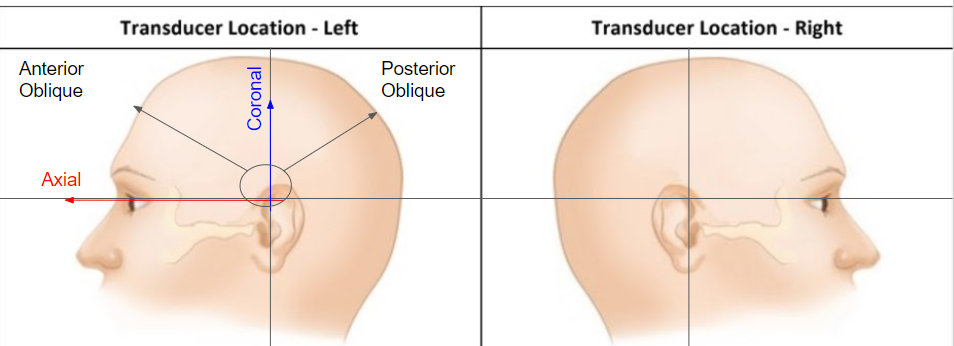
\includegraphics[width=1\linewidth]{figures/ultrasound_angle.png}
  \caption{The planes at which ultrasound data are collected: left or right side of the head and at axial, coronal, or oblique.}
  \label{ultrasound_angle}
\end{figure}

\section{Signal Processing}

Signal processing is not in the scope of my project. It was done by an ultrasound signal processing expert, Dr. John Kucewicz.
This section provide a summary of the Dr. John Kucewicz's signal processing algorithm.

Medical, diagnostic ultrasound transmits and receives short bursts of high frequency sound typically between 1 and 10 MHz. 
As sound propagates through the body, some fraction of the sound is scattered back towards the ultrasound transducer due 
to differences in local acoustic impedance.  Because of the speed of sound in tissue is relatively constant, two-dimensional 
images of tissue structure can be created based on the amplitude of the received ultrasound and the time between a sound 
burst’s transmission and its reception.  Images of blood or tissue velocity can be created by transmitting 2 or more bursts 
of ultrasound and measuring the spatially localized relative temporal shifts in the received ultrasound from burst to burst.  
In ultrasound parlance, images of structure are referred to as B-Mode, i.e. brightness mode, images, and images of velocity are 
referred to a Doppler ultrasound or tissue Doppler ultrasound if tissue velocity is being measured.

Tissue Pulsatility Imaging (TPI) is a variation of tissue Doppler designed to measure the naturally occurring pulsatile motion 
of tissue due to blood flow \cite{kucewicz_functional_2007, kucewicz_tissue_2008}.  During systole, blood accumulates in the arterial vascular causing 
tissue to expand by a fraction of a percent. Later in the cardiac cycle, accumulated blood flows through the capillary bed into 
the venous vasculature and back towards the heart allowing tissue to relax to its pre-systolic blood volume.  TPI was inspired 
by plethysmography, an older technology used to measure gross changes in tissue blood volume in, for example, an entire limb.  
TPI extends this idea to measure local changes in tissue blood volume within the body.

For this project, it is hypothesized that TPI can be used to detect variations in tissue pulsatility localized to areas of the 
brain experiencing hemorrhage.  The measurement of the TPI signal is based on standard ultrasound signal processing methods 
\cite{evans_chapter_2000}.  Ultrasound data was collected with a Terason (Burlington, MA) u3200T tablet-based ultrasound system 
and 4V2 phased-array ultrasound transducer.  With functionality enabled by the manufacturer, we were able to collect 8 seconds 
of raw ultrasound data at 30 frames per second for offline analysis in MATLAB (The Mathworks, Natick, MA).  The ultrasound data 
was filtered into 8 frequency sub-bands, quadrature demodulated, lag 1 autocorrelation was used to compute the velocity for 
each sub-band, and the velocities were averaged weighted by the power of the sub-band yielding an 8 second velocity waveform 
for every pixel in the image sequence.

Following the velocity calculation, an unpublished vector Doppler method was used to suppress common-mode motion introduced by 
gross motion of the ultrasound transducer relative to the patient. Tissue displacement was calculated from the time integral of 
velocity combined with a band-pass filter to emphasize cardiac pulsatility.  Lastly, individual cardiac cycles within the 8 seconds 
were detected and resampled such that all cycles were of uniform duration. i.e. 30 samples per cardiac cycle. Figure 
\ref{signal_processing} summarizes the signal processing steps.

\begin{figure}
  \centering
  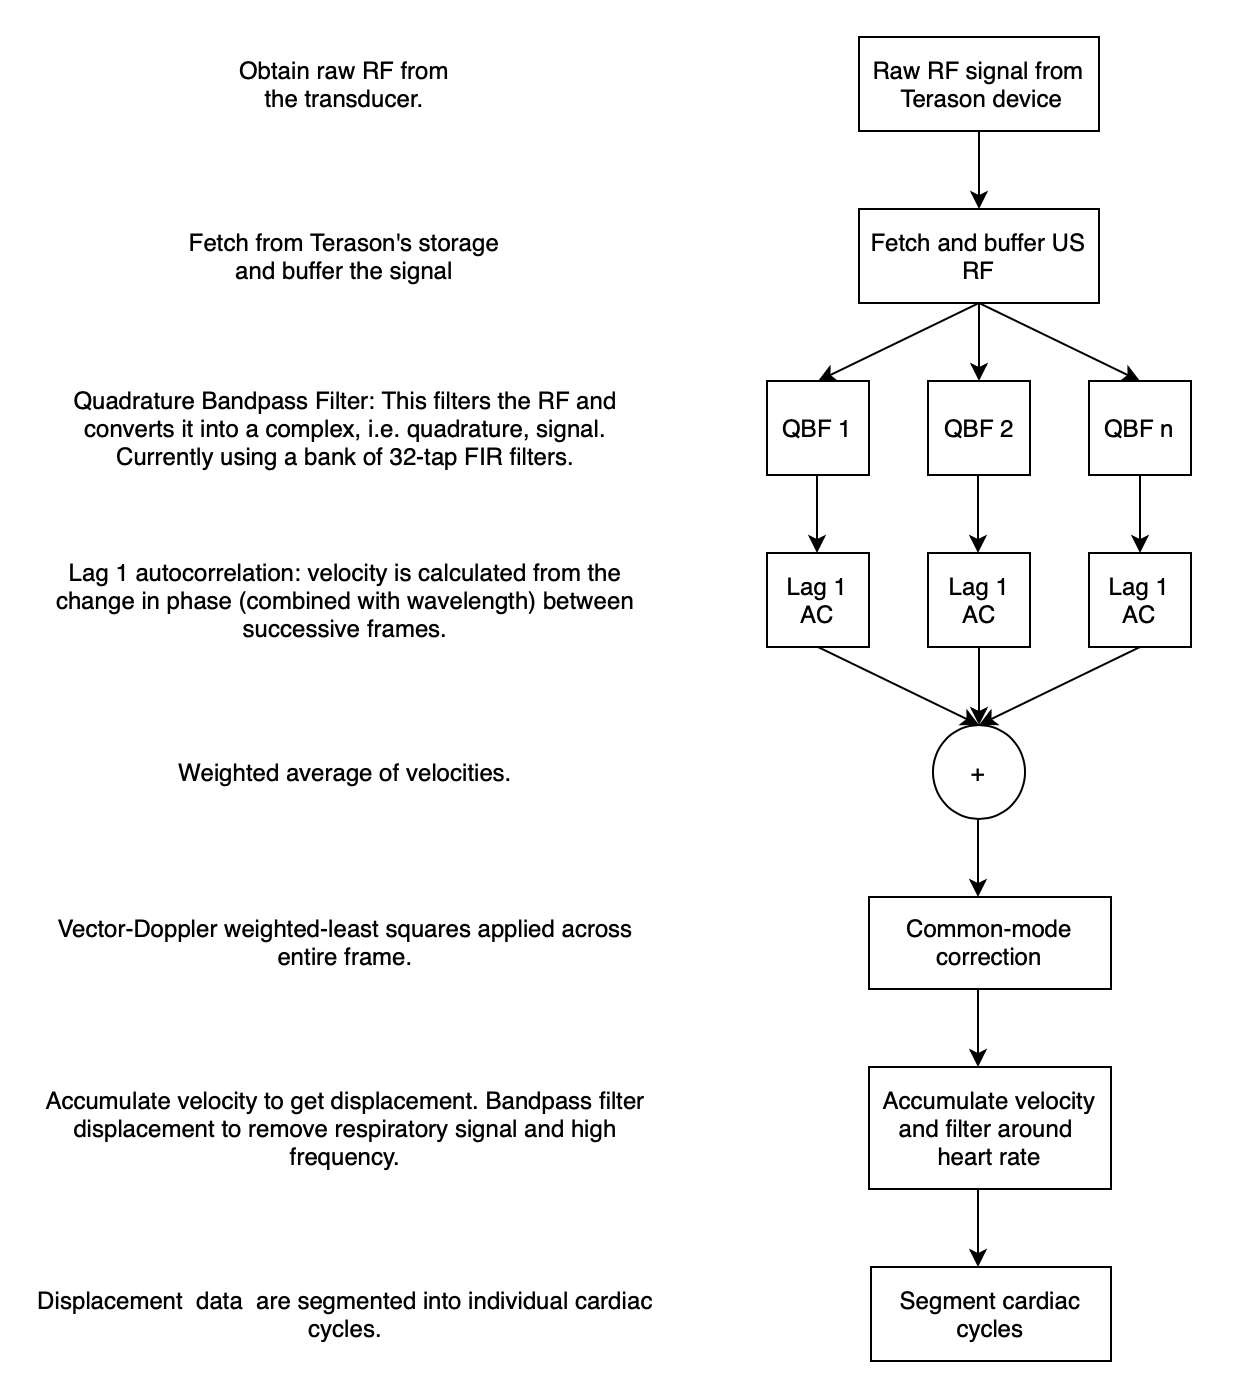
\includegraphics[width=0.9\linewidth]{figures/signal_processing.png}
  \caption{The raw RF data are processed using various signal processing techiques to produce displacement data that is synchronized 
  with the heart's cardiac cycle.}
  \label{signal_processing}
\end{figure}


\section{CT Registration to Create Masks}

TBD

\begin{figure}
  \centering
  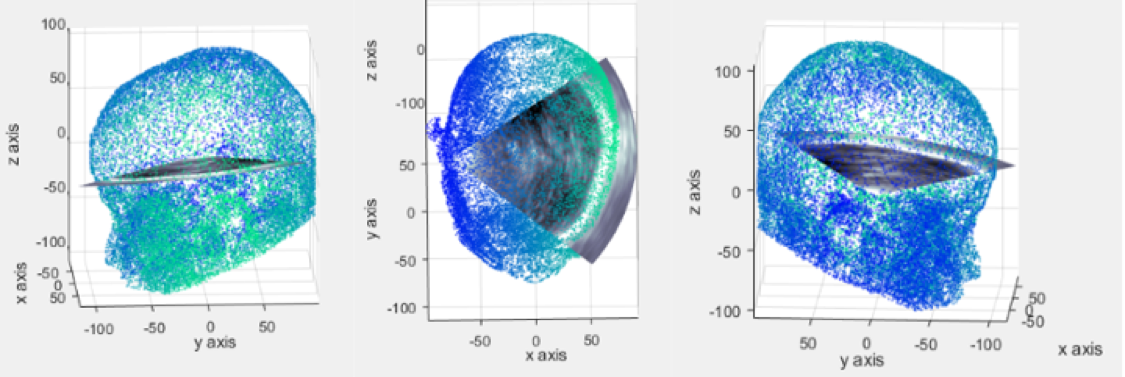
\includegraphics[width=0.9\linewidth]{figures/registration.png}
  \caption{Registering a 2D ultrasound scan plane to the 3D CT data. The 2D B-mode scane is shown relative to a point cloud representing 
  the skin surface of the head in the 3D CT data.}
  \label{registration}
\end{figure}

\begin{figure}
  \centering
  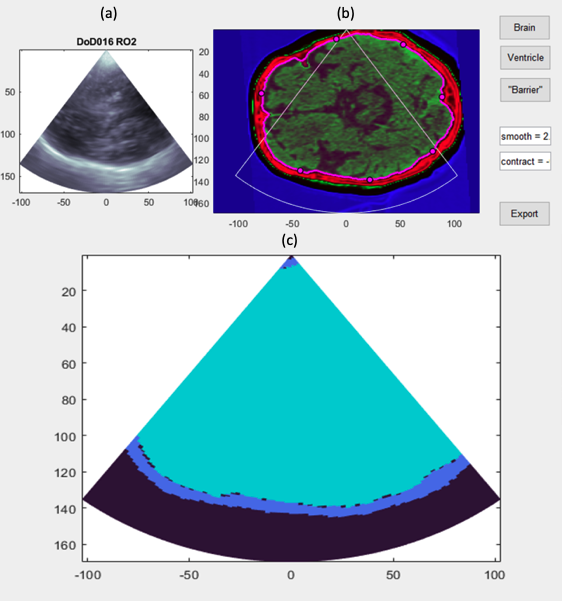
\includegraphics[width=0.6\linewidth]{figures/registration_output.png}
  \caption{CT brain mask constructed by registration with B-Mode ultrasound for patient \# 16 at the right oblique plane. 
  (a) B-mode ultrasound data. (b) An overlay of the ultrasound plane on the CT image. 
  (c) Resulting brain mask (cyan) and skull mask (blue).}
  \label{registration_output}
\end{figure}


\section{Existing System}

A previous student approached the problem of detecting intracranial hemorrhage using a different representation of 
tissue displacement data, whose description is not in the scope of this writing. The student attempted several different 
deep learning models, including MobileNetV2 \cite{sandler_mobilenetv2_2019}, pix2pix \cite{isola_image_image_2018}, 
and ResNeSt \cite{zhang_resnest_2020}. The architectures of the mentioned models were used unmodified. The loss function used for model 
optimization was categorical loss entropy. The metrics used for evaluation are precision and recall. The best model 
was reported to be ResNeSt. with a reported precision score of about 0.07 and recall of about 0.2 after 70 training epochs.

The evaluation results showed that the previous deep learning methods and data preprocessing might not be suitable for the 
detection of intracranial hemorrhage from displacement data. In addition, the choice of loss function and evaluation metrics 
is poor. Categorical loss entropy considers the predicted results of all pixel an image equally. The result is that the loss 
value could be very low, but the predictive power for a class of interest is very low. The precision and recall scores evaluate 
the quantity of true positive, true negative, false positive, and false negative in relation to each other, but they do not 
indicate how well a model learn the correct label of a pixel or how well the ground truth overlaps with the detected area.

\section{Problem Statement and Scope}
This capstone project focuses on the core algorithm that detects the regions of intracranial
hemorrhage with in a patient's brain tissue. The scope is limited to data preprocessing, skull detection,
ventricle detection, brain mass detection, and intracranial hemorrhage diagnosis.

\subsection{Data Preprocessing}

TBD

\subsection{Skull Detection}

TBD

\subsection{Brain Mass Detection}

TBD

\subsection{Hemorrhage Diagnosis}

TBD


% ========== Chapter 2

\chapter {Related Work}

\section{Overview}
Medical image segmentation aims to identify structures such as organs or lesions in 
an image; it plays a key role in computer aid diagnosis. The two categories of image 
segmentation tasks are semantic segmentation and instant segmentation \cite{lei_medical_2020}. 
Semantic segmentation involves pixel-level classification, assigning a corresponding category 
for each pixel in an image. Instant segmentation is more complex, distinguishing instances 
on the basis of specific categories in addition to outputting the basic semantic segmentation’s 
result. This project focuses on semantic segmentation; for the remaining sections of 
this writing, image segmentation means semantic segmentation. Depends on the availability 
of labeled data, different flavors of deep learning (or general machine learning) 
could be applied to solve a problem, supervised learning, weakly supervised learning, 
and unsupervised learning. When the data are carefully labeled, supervised learning 
is the popular choice. The disadvantage of this method is that it is difficult to obtain 
a large number of labeled medical images. Unsupervised learning does not require labeled 
data but the difficulty of learning is significantly higher. On the other hand, when a 
dataset contains both labeled and unlabeled images, weakly supervised learning is another 
option. Deep learning has been used widely for medical image segmentation with 
huge success compared to early approaches, including edge detection, template matching 
techniques, statistical shape models, active contours, etc \cite{lei_medical_2020}. 
This chapter discusses the recent progress in the field of medical image segmentation. 
The discussion focuses on the applications of deep-learning based medical image segmentation, 
supervised deep learning techniques, and data augmentation.

\section{Application}

Popular medical image segmentation tasks includes, but not limited to, liver 
and liver-tumor segmentation \cite{ li_automatic_2015, vivanti_automatic_nodate}, 
brain and brain-tumor segmentation \cite{menze_multimodal_2015, cherukuri_learning_2018}, 
optic disc segmentation \cite{ cheng_superpixel_2013, fu_joint_2018}, cell 
segmentation \cite{navab_u-net_2015, song_dual-channel_2017}, lung segmentation 
and segmentation of pulmonary nodules \cite{ wang_central_2017, onishi_multiplanar_2019}. 
The data used for medical diagnosis are commonly 2D gray scale or three-channel RBG images 
and 3D volumetric data. Deep learning practitioners get their data mostly from the four popular 
imaging modalities, X-ray, Computed Tomography (CT), Magnetic Resonance Imaging (MRI), and 
ultrasound \cite{lei_medical_2020}. When the structures of interest is at cellular scale, 
the images often come from Electron Microscopy (EM) \cite{navab_u-net_2015}.

\section{Supervised Learning}

Supervised learning is the most popular method for medical image segmentation tasks. 
This section reviews the existing methods that deep learning researchers have attempted 
to solve medical image segmentation problems. Specifically, I will discuss the two 
important components of a deep learning model, the backbone network and the network block.

\subsection{Backbone network}

The backbone network is the high-level architecture of a deep learning model. 
It draws a big picture of the way different pixel-level computational operations 
are chained together to process the input and output a segmentation map. In the 
last decade, researchers have proposed various backbone architectures for deep 
learning, U-Net, 3D Net, Recurrent Neural Network (RNN), skip connection, cascade 
of 2D and 3D models.

\paragraph{U-Net}

One of the most popular deep learning architectures in the field of general image 
segmentation is the encoder-decoder structure. U-Net \cite{ navab_u-net_2015}, 
fully convolution network (FCN) \cite{long_fully_nodate}, and Deeplab \cite{chen_rethinking_2017} 
are examples of the encoder-decoder structure. As the name suggest, encoder-decoder 
architectures have two main parts, the encoder and decoder. The encoder reduces the 
dimensions of the inputs and extracts image features while the decoder restores these 
features to the original size and output the segmentation maps. U-Net has been used 
widely for medical image segmentation and has become the benchmark for most medical 
image segmentation tasks\cite{}. Many modern architectures were inspired by U-Net 
\cite{wang_non-local_2020, zhou_unet_2020, jha_doubleu-net_2020, alom_recurrent_nodate}. 
Figure \ref{unet} shows the architecture of the U-Net. The left side of the U-Net works 
as a encoder. It consists of a series of convolutional filters that extract features 
and max pooling layers that shrink the inputs. The right side is the decoder that 
recovers the original image dimensions by four up-convolution operations. The U-Net 
is perfectly symmetric, allowing skip connections to concatenate the input features 
of the encoder to the features of the decoder. This structure effectively fuses 
low-level (high resolution) and high-level (low resolution) image features through 
skip connections. By these connections, the U-Net allows segmentation of medical 
images, which often contain noise and show blurred boundaries.

\begin{figure}
  \centering
  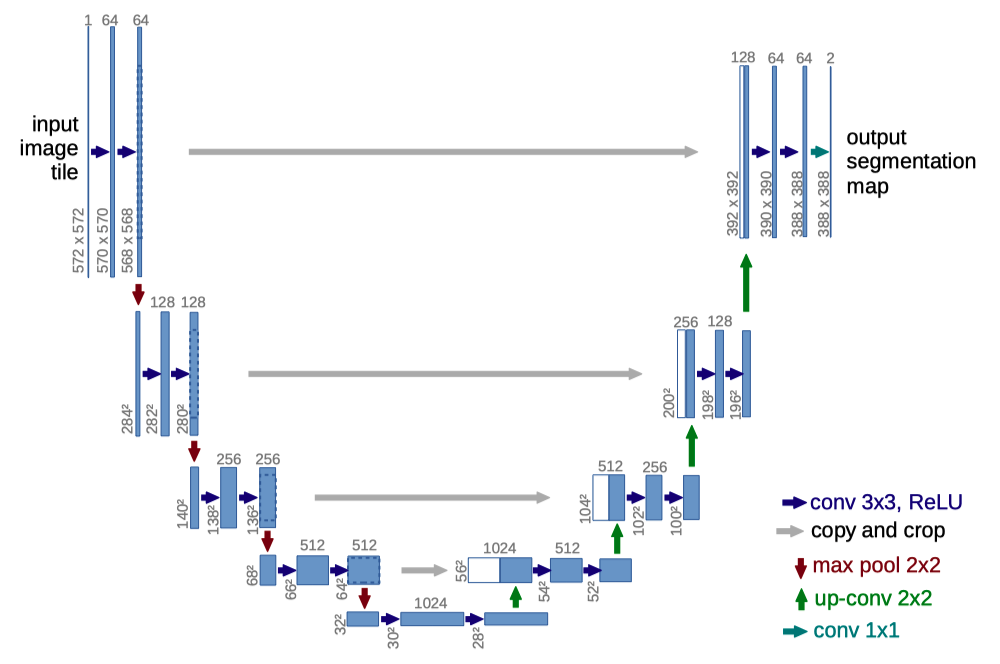
\includegraphics[width=0.8\linewidth]{figures/unet.png}
  \caption{The U-Net architecture. The left and right side are the encoder and decoder, respectively\cite{navab_u-net_2015}.}
  \label{unet}
\end{figure}

\paragraph{3D Net}

Motivated by the success of U-Net, the author of the U-Net paper extended the 
architecture to work with 3D medical data \cite{cicek_3d_2016}. Such data are 
very common in the form of volumetric CT and MRI data. Inherently, this architecture 
has more parameters and requires much higher computer resource than the U-Net. Due 
to insufficient computing capability, the authors limited the 3D U-Net to only 
three down-sampling layers, reducing the model’s segmentation accuracy when tested. 
Figure \ref{3dunet} depicts this architecture. Milletari et al. proposed a similar 
structure called V-Net, \cite{milletari_v-net_2016} as shown in Figure \ref{vnet}. 
V-Net was developed to allow stacking more network layers, providing better feature 
representation. One problem that deep neural networks face is vanishing gradient 
\cite{he_deep_2015}. The gradients (derivative) of a neural network are found using 
back propagation during the training process. By the chain rule, the derivatives of 
the hidden layers are multiplied from the output layer to the input layer to compute 
the derivative of the initial layer. If the derivatives are small, multiplication 
causes the gradient to decrease quickly, causing vanishing gradient. Residual connection 
is one of the solution for this problem \cite{he_deep_2015}. The residual connection 
(identity), as shown in Figure \ref{residual}, is essentially a skip connection that 
brings weights from an earlier stage to a later stage. These weights do not go through 
the activation function, so do not suffer from vanishing gradient. The V-Net employs 
residual connection in the design, allowing it to have four down-sampling layers.

\begin{figure}
  \centering
  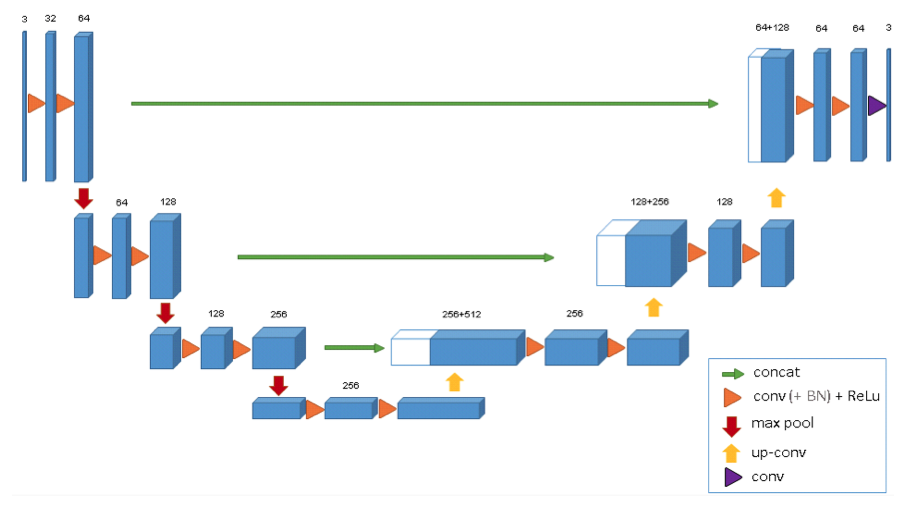
\includegraphics[width=0.8\linewidth]{figures/3dunet.png}
  \caption{The 3D U-Net architecture\cite{cicek_3d_2016}.}
  \label{3dunet}
\end{figure}

\begin{figure}
  \centering
  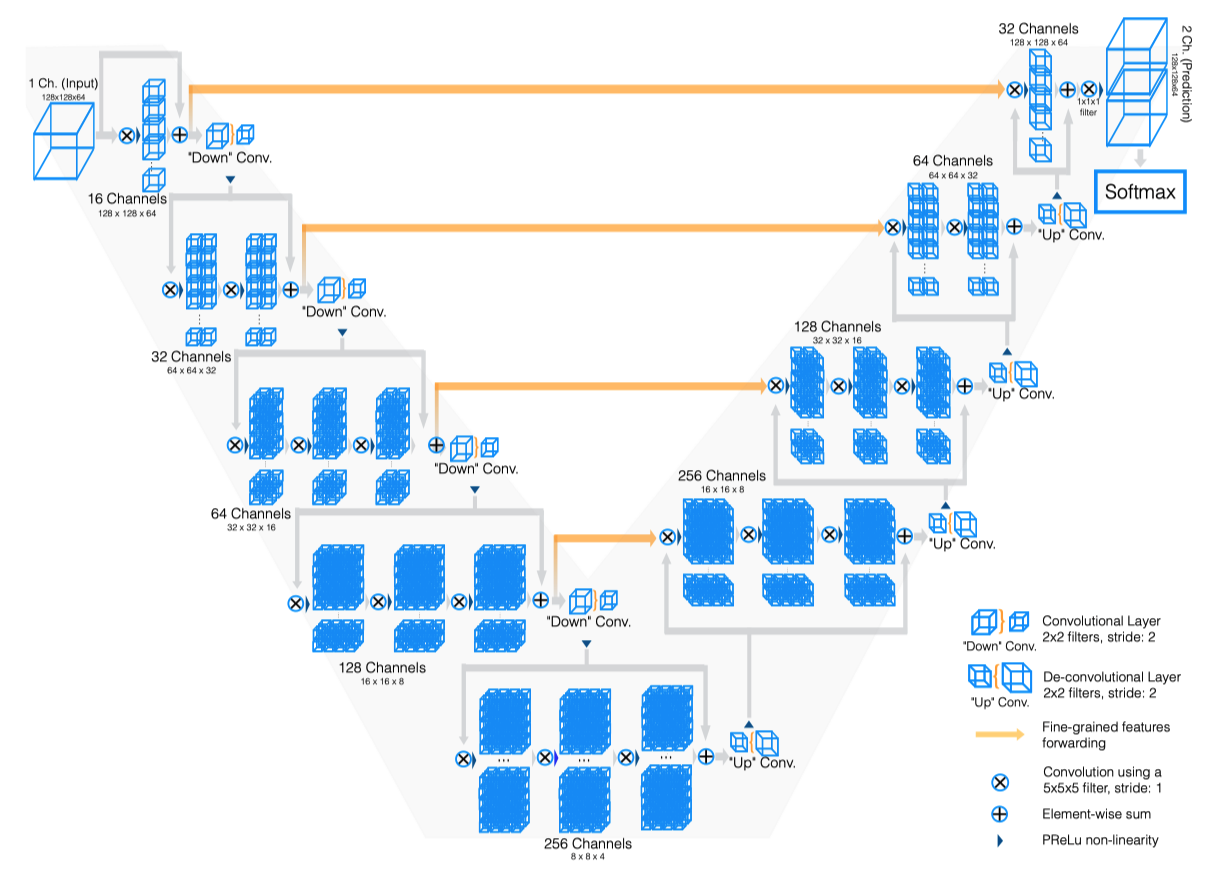
\includegraphics[width=1\linewidth]{figures/vnet.png}
  \caption{The V-Net architecture\cite{milletari_v-net_2016}.}
  \label{vnet}
\end{figure}


\begin{figure}
  \centering
  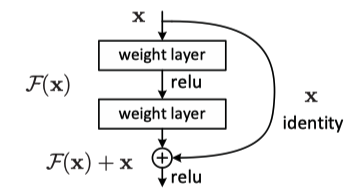
\includegraphics[width=0.4\linewidth]{figures/residual.png}
  \caption{Residual connection\cite{he_deep_2015}.}
  \label{residual}
\end{figure}


\paragraph{Recurrent Neural Network}

Recurrent neural network (RNN) is intended for sequence problems such as 
voice recognition, language translation, and time-series sequences to name 
a few. One of the most popular RNNs is the Long Short-Term Memory (LSTM) 
network, developed by Hochreiter et al. in 1997 \cite{ hochreiter_long_1997}. 
It can mitigate the vanishing gradient problem by introducing self-loop. RNN 
has been used to model the time dependence of image sequences. Alom et al. 
proposed the Recurrent Convolutional Neural Network based on U-Net (RU-Net), 
as shown in Figure \ref{rnnunet}, that improves feature representation for 
medical image segmentation tasks by recursive residual convolutional layers 
\cite{alom_recurrent_nodate}. Gao et al. proposed  the Fully Convolutional 
Structured LSTM (FCSLSTM), a combination of LSTM and CNN, to model the temporal 
relationship between different brain MRI slices \cite{gao_fully_2018}. Another 
work from Bai et al. joined FCN with RNN to extract the spatiotemporal information 
from aortic image sequences \cite{bai_recurrent_2018}.

\begin{figure}
  \centering
  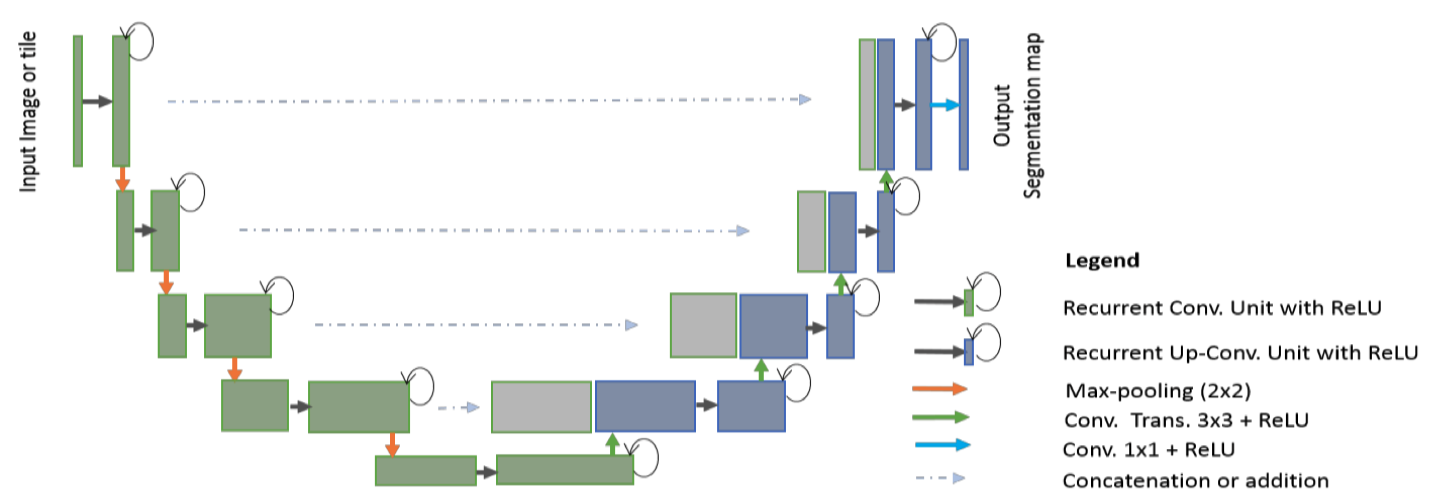
\includegraphics[width=1\linewidth]{figures/rnnunet.png}
  \caption{RU-Net architecture with convolutional encoding and decoding units using 
  recurrent convolutional layers (RCL) based on U-Net architecture.\cite{alom_recurrent_nodate}.}
  \label{rnnunet}
\end{figure}


\paragraph{Skip connection}

As aforementioned, the skip connection of U-Net fuses low-resolution and high resolutions 
features to improve feature representation. A disadvantage of the skip connection is that 
there is a large semantic gap between low-resolution and high-resolution features, leading 
to blurred feature maps \cite{ lei_medical_2020}. Ibtehaz et al. improved the original 
U-Net multiple ways, including replacing the ordinary skip connection with convolution 
operations on the encoder’s features before fusing with the decoder’s features 
\cite{ibtehaz_multiresunet_2020}. They tested the model on five different dataset, 
including EM images for cell segmentation and endoscopy images for colon cancer detection, 
and reported better performance than U-Net. Two additional work by Seo et al. \cite{seo_modified_2020} 
and Chen et al. \cite{chen_feature_2019} also added convolution operations to the skip connection 
to improve performance of liver-lesion segmentation tasks.


\paragraph{Cascade Models}

The accuracy of segmentation tasks could be improved by training multiple models and chaining 
their input/output together. This type of architecture has three main categories, coarse-fine 
segmentation, detection segmentation, and mixed segmentation \cite{lei_medical_2020}. In this 
writing, I am interested mostly in the coarse-fine segmentation type. In coarse-fine segmentation 
networks, a cascade of two 2D networks is used. The first network provides a coarse segmentation, 
and the second network refines the coarse segmentation with details. Many researchers have 
developed this type of networks for liver and liver tumor segmentation using 3D. Christ et al. 
proposed the Cascaded fully convolutional neural networks (CFCNs) for liver and liver tumor 
segmentation\cite{christ_automatic_2016}. In their work, they used an FCN to segment the liver, 
then fed the result to a second FCN for liver tumor segmentation. Other coarse-fine segmentation 
networks for liver and liver tumor segmentation are described in \cite{ tang_dsl_2018, 
kaluva_2d-densely_2018, feng_automatic_2018}.

\subsection{Netwok Block}

Within the larger backbone network, there are the network blocks that perform the 
computations on the inputs to generate the features maps. For instance, The network 
blocks of the vanilla U-Net model are simple convolutional layers. Researchers have 
devised a variety of network blocks to effectively extract features maps within a 
larger network from medical images. In this section, I will discuss three of these 
network blocks: dense connection, inception, and attention mechanism.

\paragraph{Dense Connection}

In a dense connection network, the input of the previous layers are fed into subsequence 
layers. Guan et al. replaced the last block in a layer of the U-Net model with a dense 
block as shown in Figure \ref{dense_connection} \cite{guan_fully_2020}. They named this 
architecture fully dense UNet (FD-UNet). The architecture was showed to outperform U-Net 
for removing artifacts from reconstructed 2D photoacoustic tomography images. Zhou et al. 
\cite{zhou_unet_2020} extended this idea to the larger model as shown in Figure \ref{unetpp} 
and named the new architecture UNet++. This network contains intermediate layers and skip connections, 
resulting in a highly flexible feature fusion scheme. The downside is that the number of parameters 
is much higher than the basic U-Net due to dense connection. UNet++ outperforms U-Net in 
cell segmentation, brain tumor segmentation, liver segmentation, and lung nodule segmentation.


\begin{figure}
  \centering
  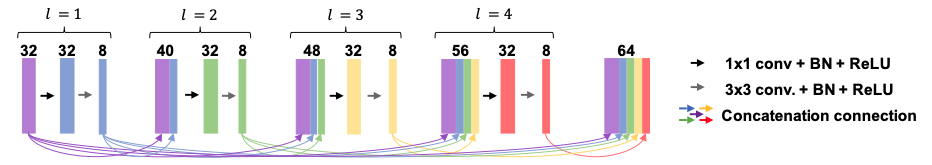
\includegraphics[width=1\linewidth]{figures/dense_connection.png}
  \caption{The dense block with four layers. The feature maps from previous layers are concatenated together as input
  to the following layers. BN stands for batch normalization \cite{guan_fully_2020}.}
  \label{dense_connection}
\end{figure}


\begin{figure}
  \centering
  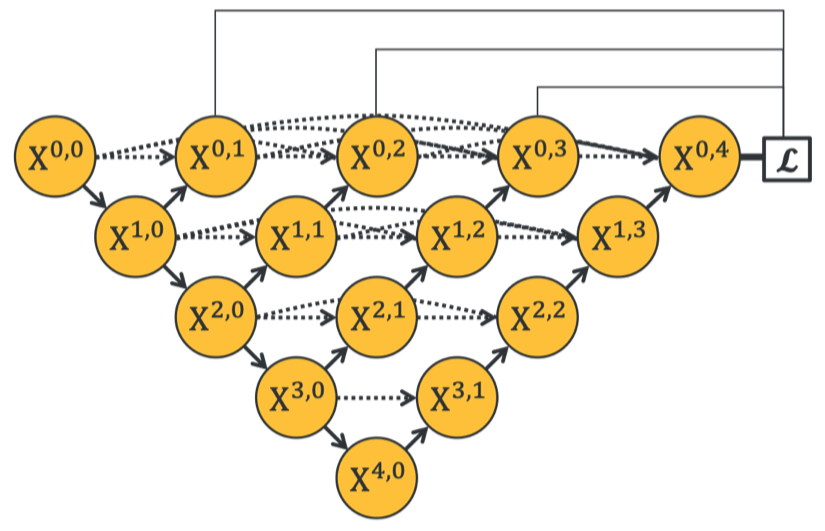
\includegraphics[width=0.6\linewidth]{figures/unet_pp.png}
  \caption{The U-Net++ architecture. Solid up and down arrows represent the encoding and decoding path,
  respectively, while dotted arrows represents skip connections. The yellow circles are
  convolutional blocks \cite{guan_fully_2020}.}
  \label{unetpp}
\end{figure}


\paragraph{Inception}

Deep CNN networks often perform better than shallows ones, but they suffer from 
problems, including vanishing gradient, difficulty of network convergence, large 
memory usage \cite{lei_medical_2020}. Gu et al. proposed CE-Net by introducing 
the inception structure into the U-Net architecture before the middle layer 
\cite{gu_ce-net_2019}. Figure \ref{dac} depicts this structure. The inception 
structure contains various atrous convolution blocks to extract features on a 
wide reception field. The inception structure improves the problems of deep CNN 
but is complex, leading to difficulty of model modification \cite{lei_medical_2020}. 

\begin{figure}
  \centering
  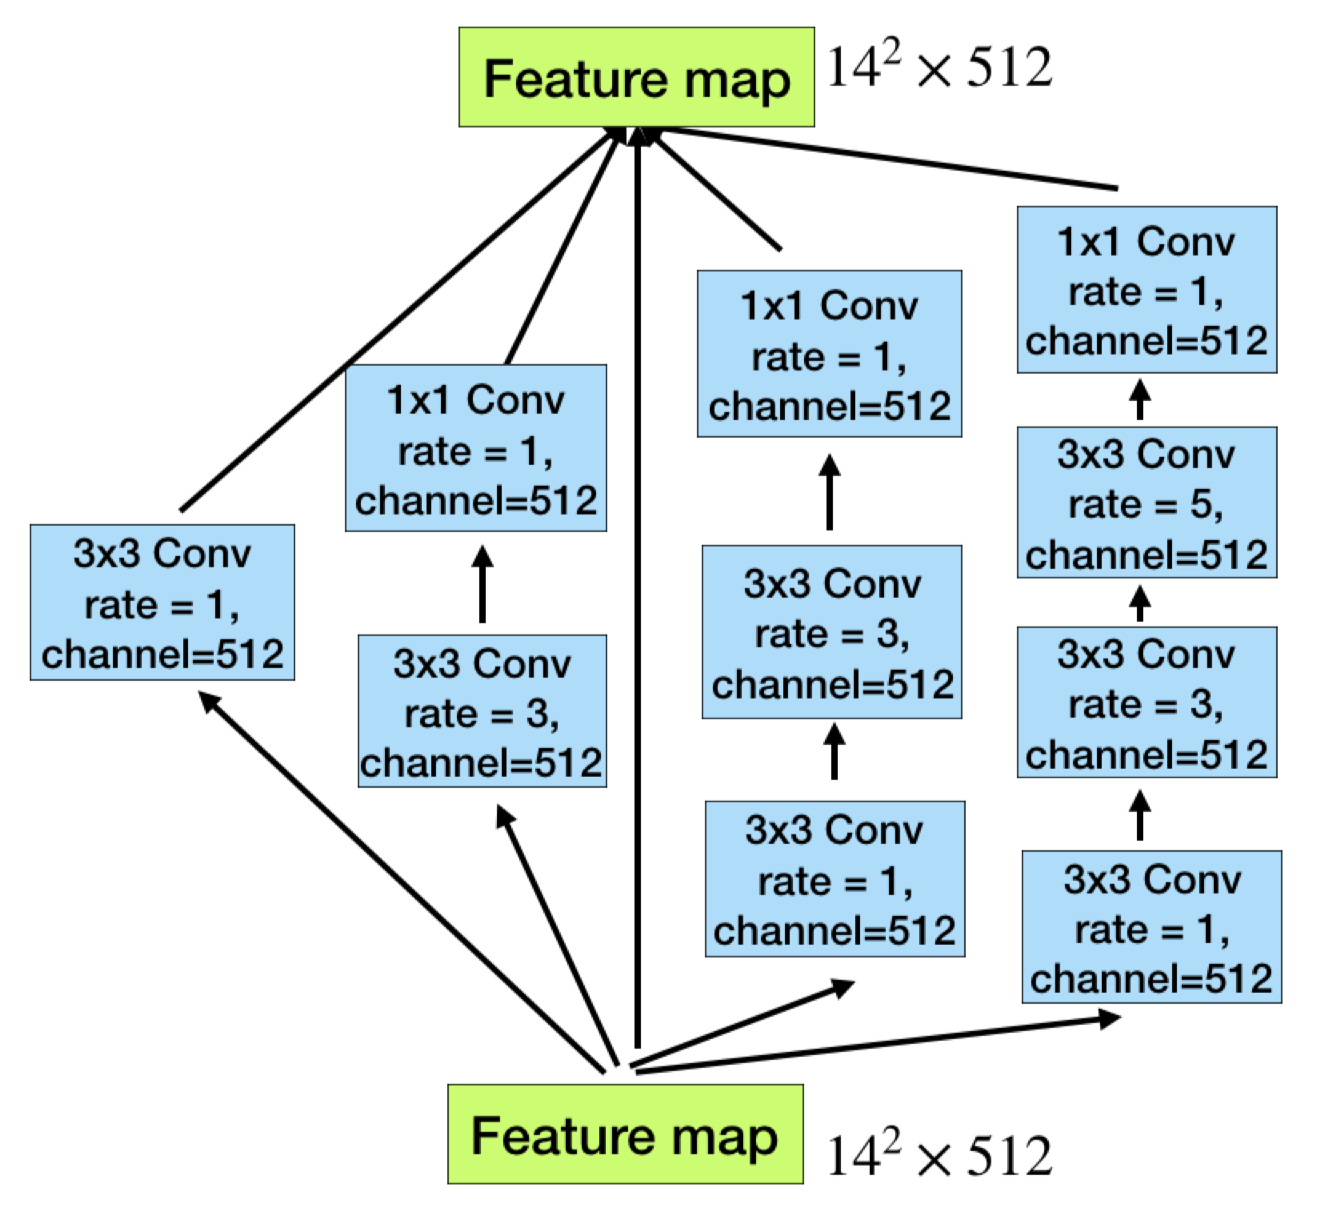
\includegraphics[width=0.6\linewidth]{figures/dense_atrous.png}
  \caption{Inception structure or dense atrous convolutional block from CE-Net \cite{gu_ce-net_2019}.}
  \label{dac}
\end{figure}


\paragraph{Attention Mechanism}

Another network block that has been shown to improve a network’s performance 
for medical image segmentation is the attention block. The basic of the attention 
block is that it can assign different weights to the input features according 
to the importance. Oktay et al. incorporated the attention mechanism into the U-Net 
and proposed attention U-Net \cite{oktay_attention_nodate}. Figure \ref{attentionUnet} 
shows the overall architecture of attention U-Net. It is very similar to the original 
U-Net besides the addition of the attention gate, as shown in Figure \ref{attentionGate}. 
This network block modifies the output of the encoder before it is concatenated 
to the decoder features. The attention gate effectively controls the feature importance 
of input pixels. 

The U-Net and many of its variations have two important limitations. The first one 
is low effectiveness: the encoder and decoder depend on local operators; the second 
is low efficiency: a large amount of feature maps are generated due to doubling of 
output channels at each step \cite{wang_non-local_2020}. Wang et al. proposed Non-local
 U-Net to solve these problems \cite{wang_non-local_2020}. Non-local U-Net contains 
 global aggregation blocks based on self-attention operator to aggregate global 
 information without a deep encoder.

\begin{figure}
  \centering
  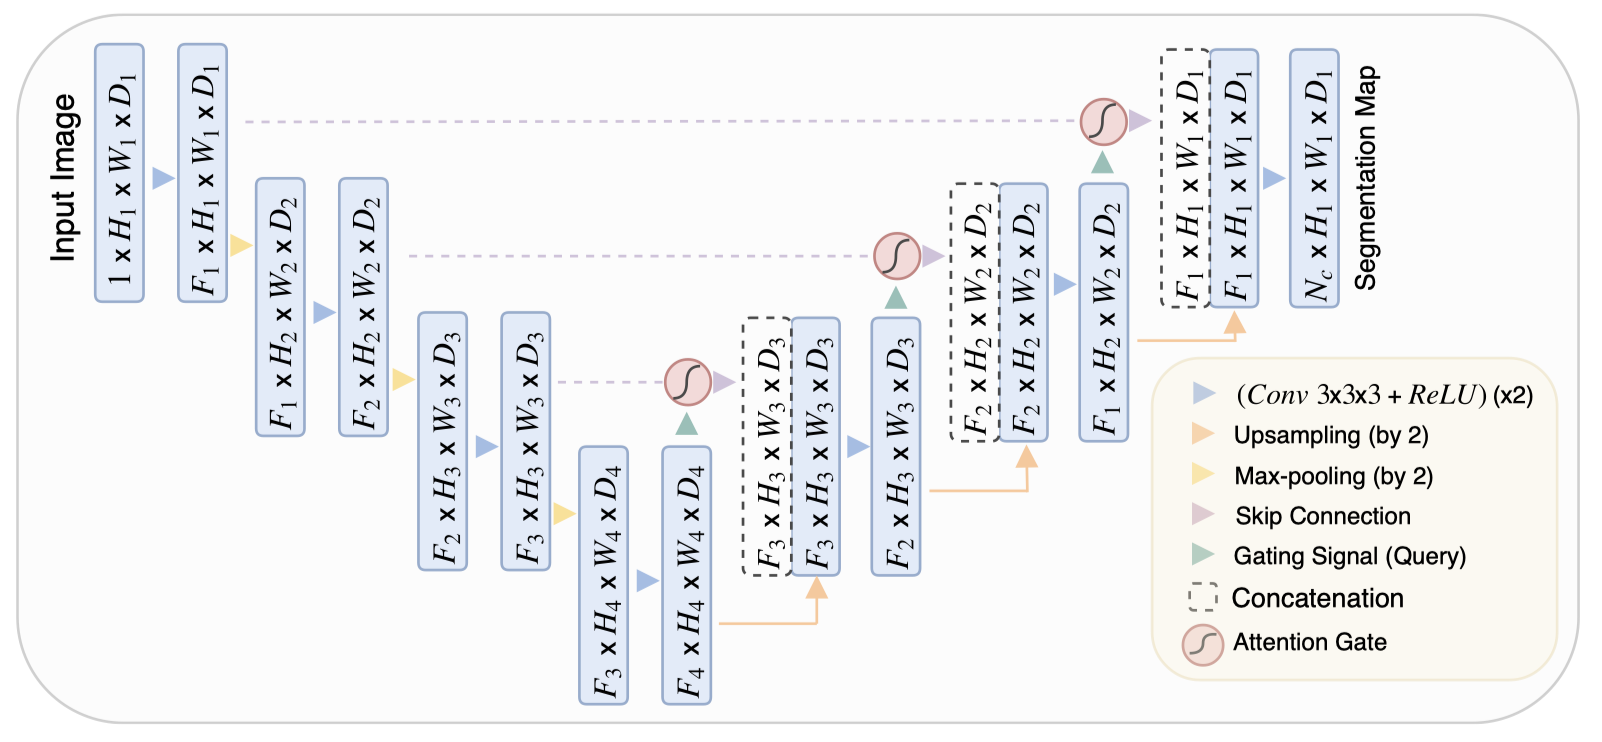
\includegraphics[width=0.8\linewidth]{figures/attentionUnet.png}
  \caption{The architecture of the attention U-Net \cite{oktay_attention_nodate}.}
  \label{attentionUnet}
\end{figure}

\begin{figure}
  \centering
  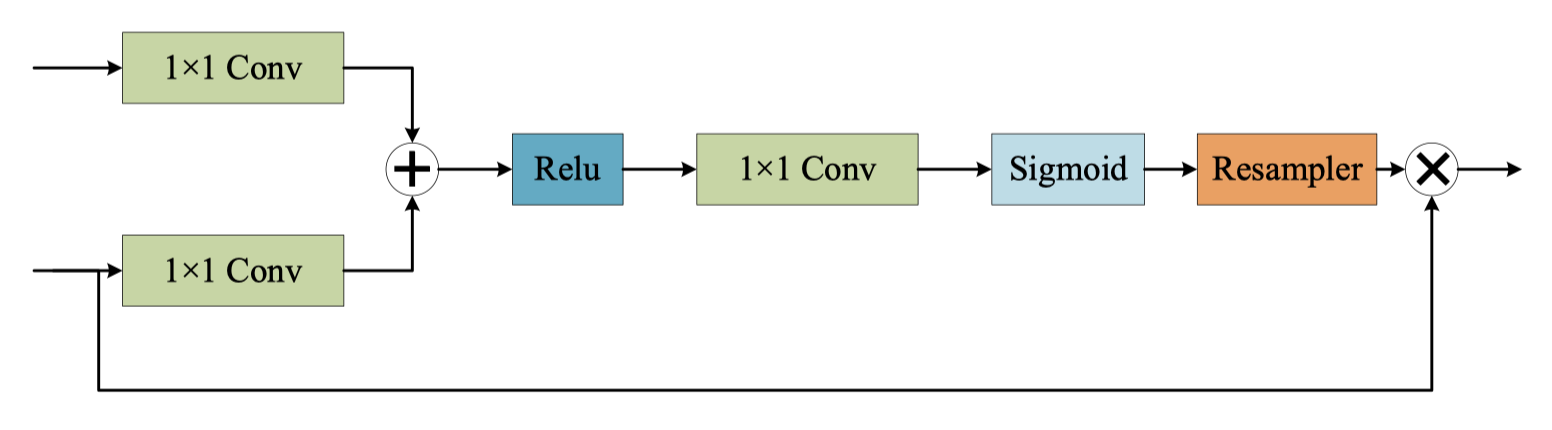
\includegraphics[width=0.7\linewidth]{figures/attentionGate.png}
  \caption{Attention gate from Attention U-Net\cite{oktay_attention_nodate}, redrawn by Lei et al. \cite{lei_medical_2020}.}
  \label{attentionGate}
\end{figure}


\subsection{Data Augmentation}

The quality of the data dictates the segmentation results of deep learning models. However, 
in the medical field, it is difficult to build high-quality datasets since the cost of data 
acquisition and labeling is very high \cite{lei_medical_2020}. In the absence of large 
labeled datasets, researchers have to rely on data augmentation. Conditional generative 
adversarial nets (cGAN) is frequently used to generate additional data for various medical 
segmentation tasks. Guibas et al. proposed an architecture that contains a GAN and a cGAN 
to generate synthetic images of retinal fundi images \cite{guibas_synthetic_2018}. Another 
work by Mahapatra et al. employed a cGAN to synthesize realistic chest X-ray images with 
different disease characteristics by conditioning the model on real samples 
\cite{mahapatra_efficient_2018}.


% ========== Chapter 3

\chapter {Method}

\section{Data and Preprocessing}






% ========== Chapter 4

\chapter {Experiment and Result}




% ========== Chapter 5

\chapter {Conclusion and Future Work}

\section{Conclusion}



\section{Limitation}
Talk about the unique differences of bTBI and other cTBI as point out in this 
paper \cite{explosive} and that data available to the study are related to 
cTBI instead of bTBI.

From an interview with the sonographer on the team, one of the many difficulties in this
study is that the team do not know the exact time of the injury. If the more data could be
collected, she believes that it would be best if data were collected as soon as possible after
a patient is admitted. This way, the data would be "fresh", more representative of the data that
would be scanned by the medics on the battle field.


\section{Future work}


 
 
 
 
%%  
%% \section{Customization of the Macros}
%%  
%% Simple customization, including 
%% alteration of default parameters,  changes to dimensions,
%% paragraph indentation, and margins, are not too difficult.
%% You have the choice of modifying the class file ({\tt uwthesis.cls})
%% or loading
%% one or more personal style files to customize your thesis.
%% The latter is usually most convenient, since you do not need
%% to edit the large and complicated class file.
%% 
 

%
% ==========   Bibliography
%
\nocite{*}   % include everything in the uwthesis.bib file
\bibliographystyle{plain}
\bibliography{uwthesis}
%
% ==========   Appendices
%
\appendix
\raggedbottom\sloppy



\end{document}
